\documentclass{article}
\usepackage{amsmath}
\usepackage{graphicx}
\usepackage{hyperref}
\usepackage{physics}
\usepackage{tikz}
\usepackage{amsfonts}
\usepackage[most]{tcolorbox}
\usepackage[utf8]{inputenc}
\usetikzlibrary{calc}
% \usepackage[dvipsnames]{xcolor}

\definecolor{block-gray}{rgb}{0, 0.8, 0}
\newtcolorbox{answer}{colback=block-gray,grow to right by=-10mm,grow to left by=-10mm,
boxrule=0pt,boxsep=0pt,breakable}

% \graphicspath{ {images/} }
 
\title{Research 1}
\author{Lev Kozlov}
\date{September 2022}

\begin{document}

\maketitle

\subsection*{Tools}

\begin{itemize}
      \item Python
      \item Numpy, matplotlib
\end{itemize}

\section*{Solution}

\href{https://github.com/lvjonok/f22-theoretical-mechanics/blob/master/research1/main.ipynb}{Source code}

\begin{enumerate}
      \item Introduce basic equations:
            \begin{align}
                  y = A \sin(O_m x + \theta_0) \\
                  y'_x = A O_m \cos(O_m x + \theta_0)
            \end{align}
            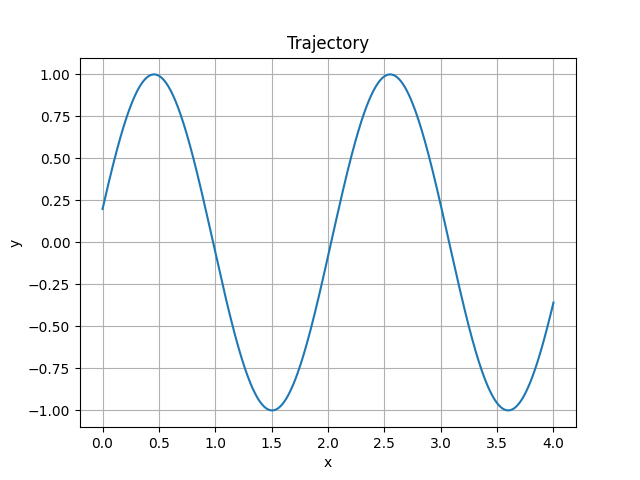
\includegraphics[width=\linewidth]{trajectory.png}
      \item Find natural form of motion:
            \begin{align}
                  \sigma(x) = \int_{X_{min}}^{x} \sqrt{1 + {y'_{x}(x)}^2} dx \\
                  \dot{\sigma}(x) = \sqrt{1 + {y'_{x}(x)}^2}
            \end{align}
      \item As we prepared inital formulas, we can proceed with explanations.
      \item Find how limitation on normal acceleration affects the motion.
            \begin{enumerate}
                  \item Curvature formula:
                        \begin{align}
                              \kappa(x) = \frac{|y''_x(x)|}{\sqrt{1 + {y'_{x}(x)}^2}}
                        \end{align}
                  \item Let us imagine we are moving with $v_{max}$, what our normal acceleration would be throughout the x
                        \begin{align}
                              a_n(x) = v_{max}^2 \kappa(x)
                        \end{align}
                        % insert graph here
                        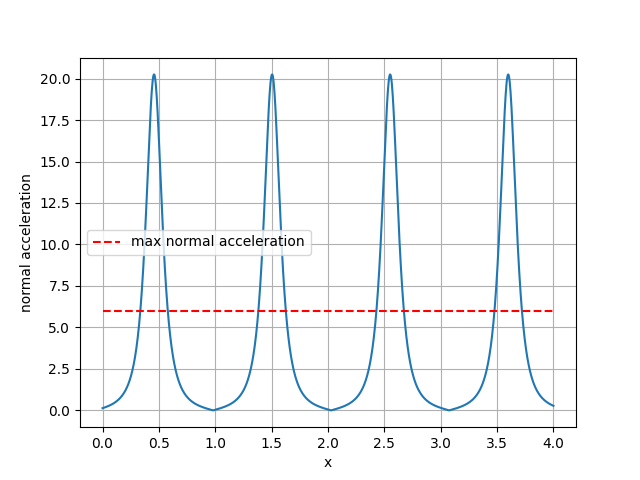
\includegraphics[width=\linewidth]{normal_acceleration_lim.png}
                  \item As we see that normal acceleration exceeds the limitation,
                        we could reverse calculations and obtain the maximum velocity we could take through the curve.
                        \begin{align}
                              v_{max}(x) = \sqrt{\frac{a_n(x)}{\kappa(x)}}
                        \end{align}
                        % insert graph here
                        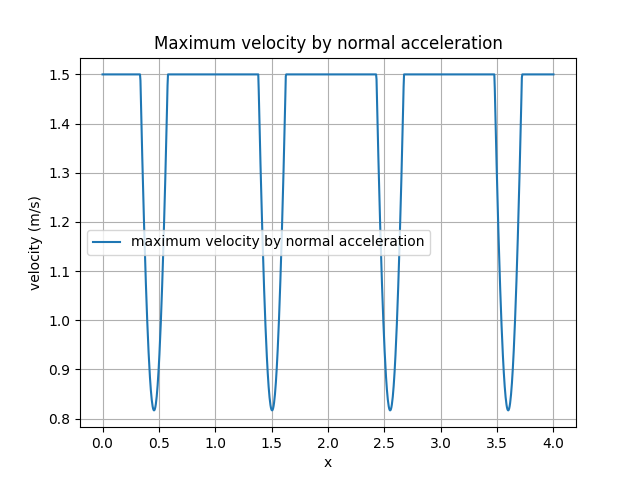
\includegraphics[width=\linewidth]{velocity_by_normal_acceleration.png}
            \end{enumerate}
      \item Find how limitation on tangential acceleration affects the motion.
            \begin{enumerate}
                  \item We can observe that at some point we cannot accelerate and decelerate on the given $dx$ interval.
                        I would thank Ilya Miloshin for explanation of this case.
                        \begin{align}
                              a_{\tau}(t) = \frac{v'_{max}(x(\sigma(t)))}{dt} = \frac{dv_{max}}{dx} \frac{dx}{d\sigma} \frac{d\sigma}{dt} \\
                              \frac{dx}{d\sigma} = \frac{1}{\sqrt{1 + {y'_{x}}^2}}
                        \end{align}
                  \item Actually, the difference between velocity limited by
                        normal acceleration and further by tangential component was not big. \\
                        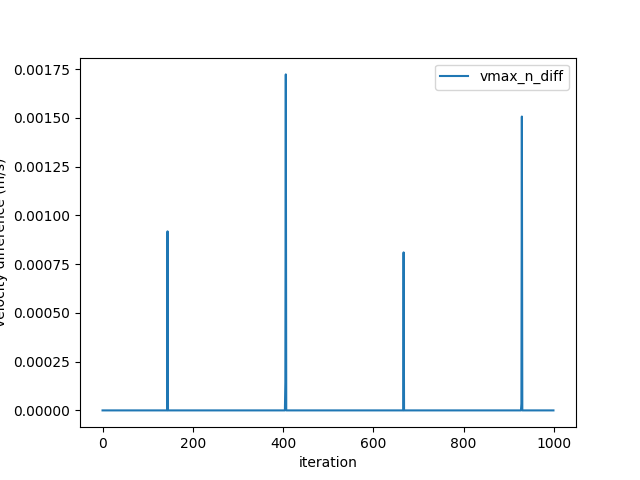
\includegraphics[width=\linewidth]{veldiff.png}
            \end{enumerate}
      \item Tangential acceleration \\
            By differentiating the velocity by x, we can find the tangential acceleration for each x. \\
            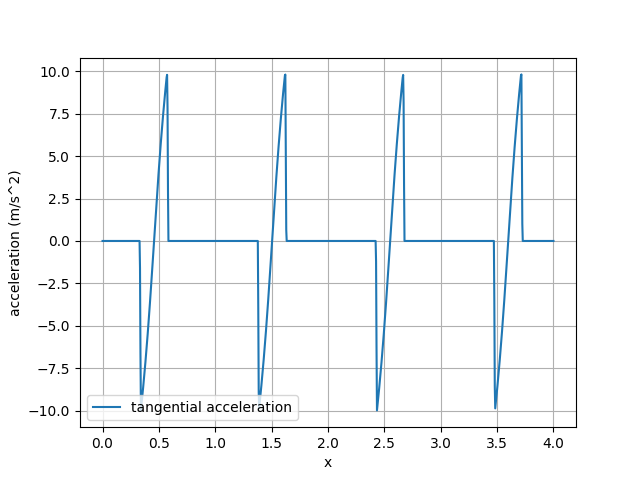
\includegraphics[width=\linewidth]{acctan_x.png}
      \item Acceleration and deceleration \\
            So far there was no talk about start and finish of trajectory.
            \begin{enumerate}
                  \item We have to start from 0 velocity and end with 0 velocity.
                  \item We will use trapezoidal profile during simulation to accelerate and decelerate.
                  \item Position to start deceleration:
                        \begin{align}
                              t_{decel} = \frac{v_{max}}{a_{\tau}} \approx 0.15 \\
                              s_{decel} = a_{\tau max} * t_{decel}^2 / 2
                        \end{align}
                  \item So, when we are left with $s_{decel}$ distance (we will convert to $x_{decel}$ for simplicity in code),
                        we start deceleration.
            \end{enumerate}
      \item Simulation \\
            \begin{enumerate}
                  \item We will use trapezoidal profile for acceleration and deceleration
                  \item General approach:
                        \begin{enumerate}
                              \item Choose appropriate acceleration
                              \item Store current parameters to use in next iteration
                              \item Velocity simulation:
                                    \begin{align}
                                          v(t) = v(t - dt) + a(t) \cdot dt
                                    \end{align}
                              \item Position simulation:
                                    \begin{align}
                                          x(t) = x(t - dt) + v(t) \cdot dt \cdot \Big( \sqrt{1 + {y'_{x}}^2}\Big)^{-1}
                                    \end{align}
                                    Multiplication by $\dot{\sigma} (x)$ is done to consider only $x$ part of position change change.
                              \item Y coordinate can be just taken for particular $x$ from trajectory.
                              \item Normal acceleration can be calculated through current velocity and x coordinate:
                                    \begin{align}
                                          a_n(t) = v(t)^2 \kappa(x(t))
                                    \end{align}
                        \end{enumerate}
                  \item Part 1: accelerate until velocity has reached maximum
                        \begin{align}
                              a_{\tau}(t) = a_{\tau max}
                        \end{align}
                  \item Part 2: Follow acceleration profile for $x$'s until we reach $x_{decel}$
                        \begin{align}
                              a_{\tau}(t) = a_{\tau}(x_{cur})
                        \end{align}
                  \item Part 3: decelerate until velocity has reached 0
                        \begin{align}
                              a_{\tau}(t) = -a_{\tau max}
                        \end{align}
            \end{enumerate}
\end{enumerate}

\begin{center}
      \makebox[\textwidth]{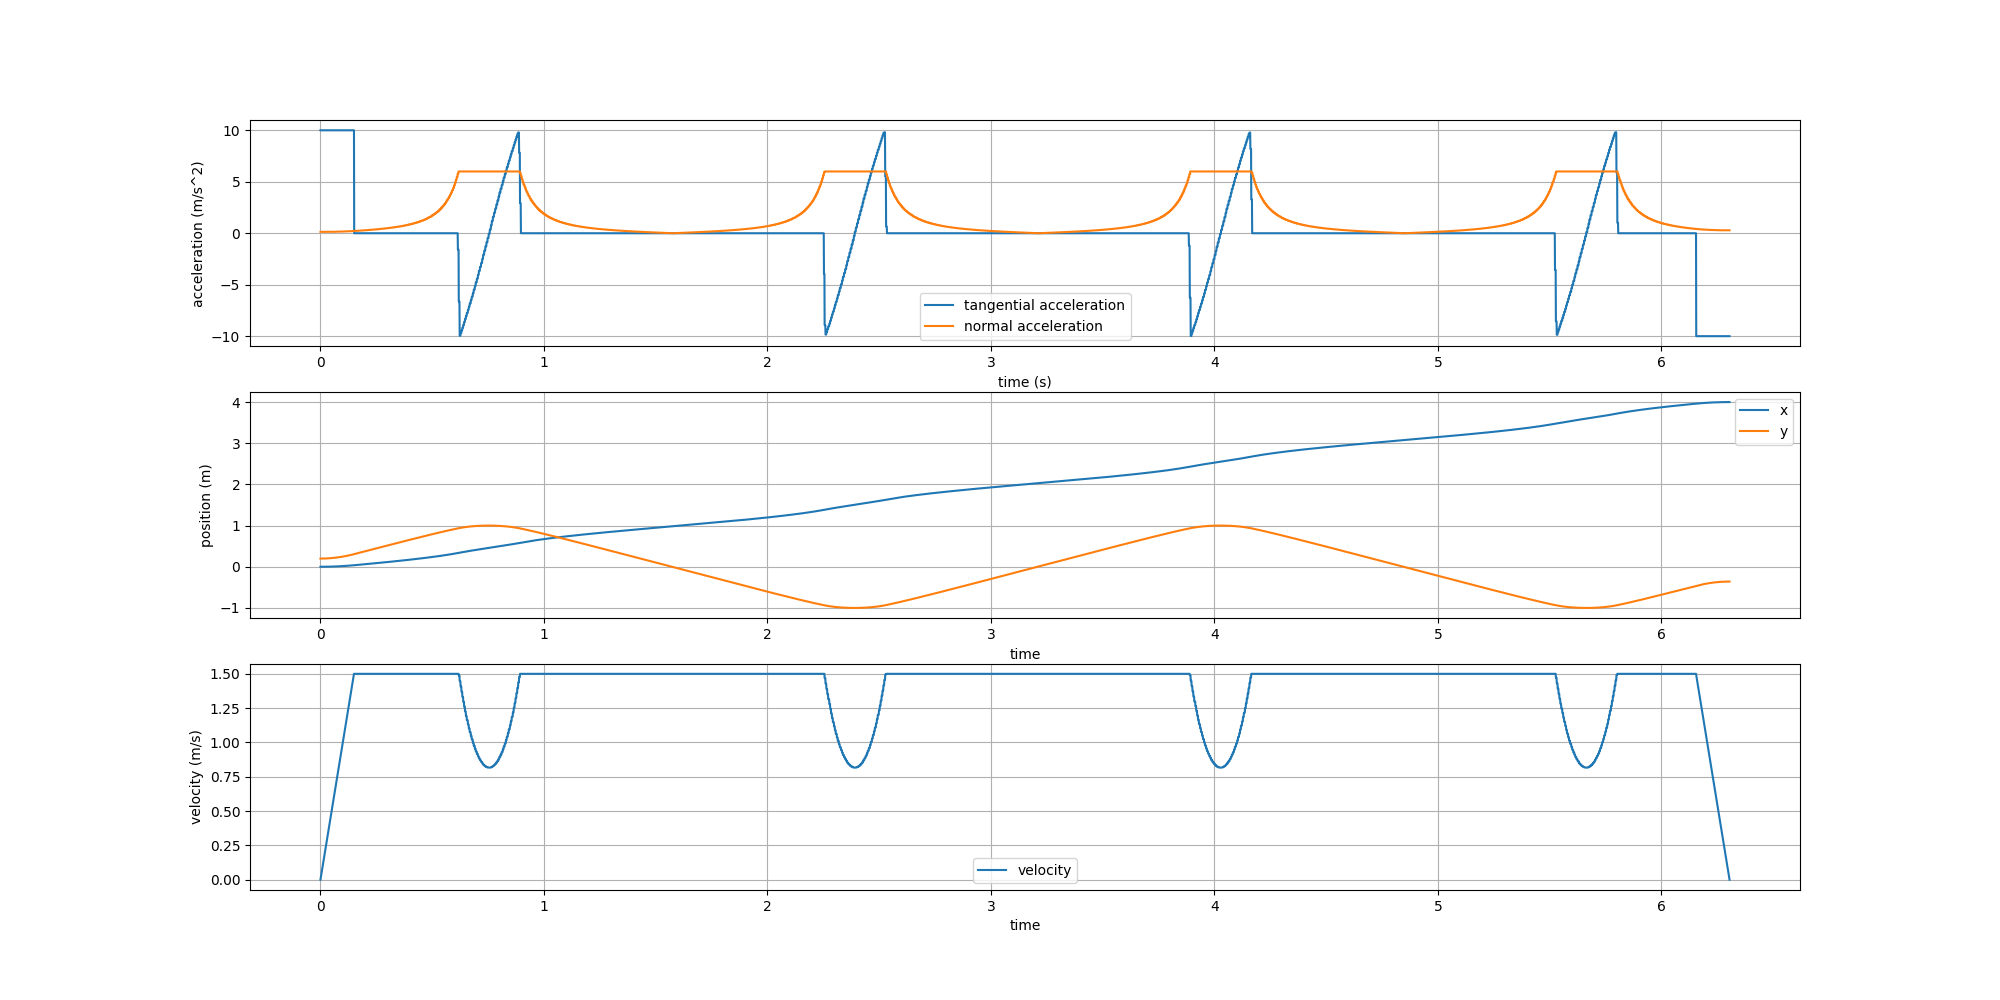
\includegraphics[width=\paperwidth]{result.png}}
\end{center}

\subsection*{Answer:}

\begin{answer}
      For my simulation approximate time to follow this trajectory was: 6.3 seconds.
\end{answer}

\end{document}